\documentclass{article}

\usepackage{corl_2026}
\usepackage{amsmath}
\usepackage{amssymb}
\usepackage{bm}
\usepackage{booktabs}
\usepackage{array}
\usepackage{graphicx}
\usepackage{textcomp}
\usepackage{algorithm}
\usepackage{algpseudocode}
\usepackage{multirow}
\usepackage{url}
\usepackage{placeins}
\usepackage{hyperref}
\title{Energy-Aware Target Streams for Learned Fixed-Wing Maneuvering}

\author{Anonymous Authors}

\newcommand{\vt}{v_t}
\newcommand{\R}{\mathbb{R}}

\begin{document}
\maketitle

%===============================================================================

\begin{abstract}
Despite rapid progress in learning-based multirotor control, learned fixed-wing maneuvering remains comparatively underdeveloped because fixed-wing aircraft must execute maneuvers through coupled attitude, lift, velocity, energy, and actuator-limited dynamics rather than hover-like position regulation.
We address this gap with \emph{energy-aware target streams}, a framework that learns a direct-actuator attitude--speed flight skill, expands its vertical maneuvering capability through energy-aware PPO fine-tuning, and composes the frozen skill into long-horizon maneuvers by optimizing executable target streams rather than actuator sequences.
We first compare Euler-angle and quaternion target encodings for direct fixed-wing RL control. Euler targets remain effective on simple commands, but quaternion conditioning provides a more consistent executor for complex turning and curve-following tasks.
Geometry-aware metrics then expose \emph{pseudo-tracking}: low cross-track error can coexist with incorrect nose direction, velocity tangent, wing-plane alignment, angle of attack, or energy state.
Starting from the quaternion skill, energy-aware fine-tuning expands the reliable envelope using energy-retention, low-speed safety, vertical-progress, aerodynamic-safety, smoothness, and replay terms.
We formulate target-stream optimization as closed-loop selection over heading--pitch--roll--airspeed stream parameters, evaluated by rollout through the frozen policy and fixed-wing dynamics.
The selected streams improve CTE-P90 by 39\%, 2\%, 24\%, and 47\% on S-curve, figure-eight, helix, and $90^\circ$ vertical pull-up tasks.
With the energy-aware fine-tuned PPO executor and selected target streams, the system further completes loop-like vertical maneuvers, including a full-loop execution in simulation.
Geometry-aware evaluation shows that the remaining limitations are no longer basic maneuver completion, but execution quality, wing-plane consistency, energy margins, and sim-to-real validation.
\end{abstract}

\vspace{-0.4em}
\begingroup
\small
\setlength{\leftskip}{0.67in}
\noindent\textbf{Code:}
\href{https://anonymous.4open.science/r/Energy-Aware-Target-Streams-for-Learned-Fixed-Wing-Maneuvering-B550/}
{\texttt{anonymous.4open.science/r/Energy-Aware-Target-Streams-B550}}
\par
\endgroup
\vspace{0.3em}

\keywords{fixed-wing aerial robots, reinforcement learning, maneuver composition, target streams, closed-loop stream selection}

%===============================================================================

\section{Introduction}

Learning-based aerial control has advanced rapidly on multirotor platforms, but learned fixed-wing maneuvering remains comparatively underexplored. The gap is not only one of platform choice: fixed-wing aircraft cannot hover, stop at a waypoint, or rotate in place. Their maneuvers are governed by coupled attitude, lift, velocity direction, energy, actuator authority, and safety margins. As a result, cross-track error (CTE) alone is insufficient: a trajectory may stay close to a spatial reference while the aircraft loses energy, drifts out of the maneuver plane, or flies with inconsistent nose and velocity directions.

This paper studies learned fixed-wing maneuvering as an executable skill-composition problem. Instead of placing learning above a hand-tuned PID/autopilot inner loop, we train a direct-actuator reinforcement-learning skill that outputs throttle, elevator, aileron, rudder, and speed brake. This exposes the learned policy to the actuator limits, aerodynamic coupling, and energy loss that determine whether a maneuver command is actually executable.

Our method follows a failure-driven progression. An Euler-angle direct-RL baseline remains useful on simple targets, but degrades on complex turning and curve-following tasks. We therefore use a quaternion-conditioned attitude--speed interface as the reusable low-level skill. Geometry-aware evaluation then reveals pseudo-tracking: low CTE can coexist with poor tangent alignment, wing-plane inconsistency, unsafe angle of attack, or energy loss. To address this failure mode, we introduce energy-aware PPO fine-tuning over vertical-arc curricula, safety/energy rewards, and replay.

For long-horizon maneuvers, we do not optimize actuator sequences directly. Instead, we convert each reference maneuver into an executable stream of local heading, pitch, roll, and airspeed targets. We then select low-dimensional stream parameters by closed-loop rollout through the frozen learned skill and fixed-wing dynamics, so the chosen stream is evaluated by actual execution rather than open-loop geometric closeness.

In summary, this paper contributes: (i) a direct-actuator fixed-wing RL skill with an Euler-to-quaternion target evolution, (ii) geometry-aware metrics for pseudo-tracking diagnosis, (iii) energy-aware PPO fine-tuning for vertical and loop-like maneuver capability expansion, and (iv) executable target streams with closed-loop stream selection for long-horizon fixed-wing maneuver composition.

%===============================================================================

\section{Related Work}

\paragraph{Learning-Control Interfaces for Agile Flight.}
CoRL flight systems often place learning at an inspectable interface rather than replacing the full autonomy stack.
Deep Drone Racing maps images to waypoints and desired speeds for downstream planning and control~\citep{kaufmann2018deep}, and learning-based visual navigation combines learned perception with model-based planning and feedback~\citep{bansal2019combining}.
Our interface is different: for fixed-wing maneuvering, the executable object is an attitude--speed target stream rather than a waypoint-speed command.

\paragraph{Direct Learned Flight Control.}
Direct learned controllers have been used for swarm flight and soft multicopter control~\citep{batra2021decentralized,deng2020soft}.
For fixed-wing aircraft, PPO-based attitude controllers have been studied in simulation and field experiments~\citep{bohn2020deep,bohn2024data}.
Our policy is also direct at the actuator level, but remains target-conditioned rather than being an unconstrained end-to-end maneuver policy.

\paragraph{Fixed-Wing Guidance and Feasibility-Aware Tracking.}
Classical fixed-wing autonomy often separates path geometry, guidance, and inner-loop control.
Dubins-style paths, nonlinear guidance laws, and vector-field methods provide standard tools for curvature-constrained fixed-wing path following~\citep{dubins1957curves,park2004new,nelson2007vector,sujit2014uav}.
For agile robots, trajectory generation and receding-horizon methods reason about dynamic feasibility and finite-horizon objectives~\citep{mellinger2011minimum,mayne2000constrained,williams2017mppi,rubinstein1999cross}, while DATT and learned time-allocation methods address infeasible or actuator-limited quadrotor references~\citep{huang2023datt,ryou2022real}.
In contrast, our target-stream selection checks feasibility through closed-loop execution by a learned fixed-wing executor.

\paragraph{Simulation and Evaluation.}
Fast simulation is central to robot learning, from Flightmare for quadrotors~\citep{song2020flightmare} to general or vehicle simulators such as MuJoCo, AirSim, FlightGoggles, and JSBSim~\citep{todorov2012mujoco,shah2018airsim,guerra2019flightgoggles,berndt2004jsbsim}, as well as accelerator-oriented engines such as Brax and Isaac Gym~\citep{freeman2021brax,makoviychuk2021isaac}.
Our simulator is not the contribution of this paper; the evaluation gap addressed here is fixed-wing-specific: position error can hide invalid nose direction, velocity-tangent alignment, wing-plane orientation, energy state, angle of attack, sideslip, G-load, and termination risk.
%===============================================================================

\section{Method}

\begin{figure}[t]
  \centering
  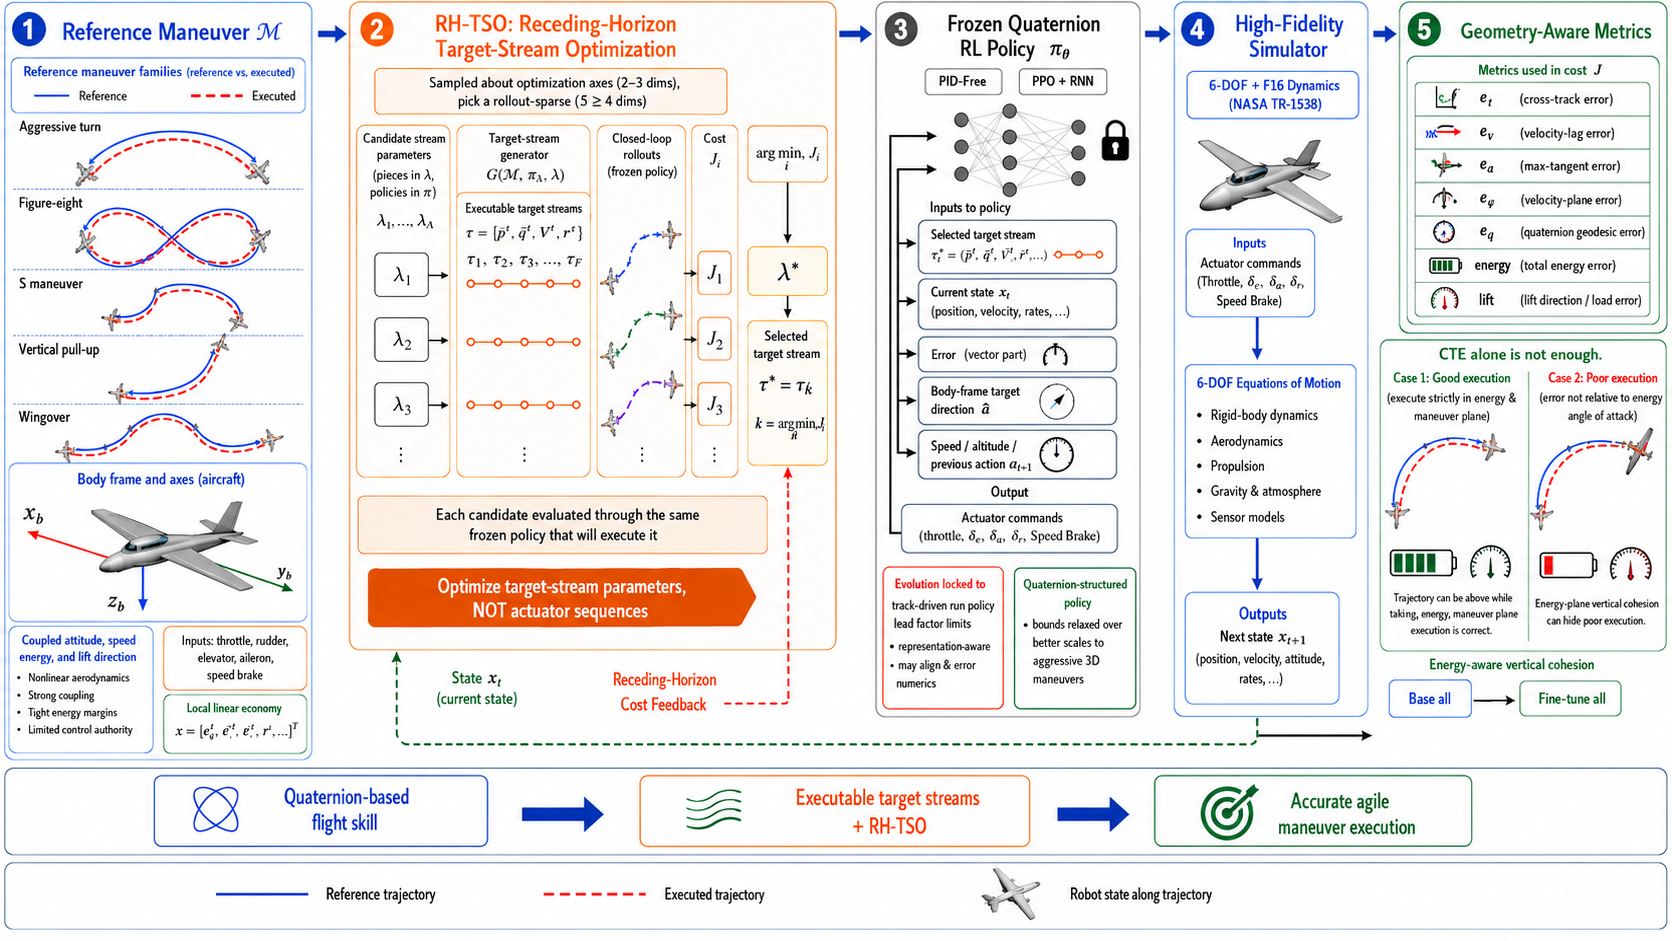
\includegraphics[width=\textwidth]{figure/figure1.png}
  \caption{\textbf{System overview.} Training expands a direct-actuator fixed-wing skill from Euler-angle targets to a quaternion-conditioned, energy-aware executor.
  A reference maneuver is converted into heading--pitch--roll--airspeed target streams, whose parameters are selected by closed-loop rollout through the frozen skill and fixed-wing dynamics.}
  \label{fig:system}
\end{figure}

The system separates the reusable flight skill from the long-horizon composition layer. The skill provides a local attitude-speed tracking interface under actuator and aerodynamic constraints. The composition layer converts reference geometry into target streams and selects stream parameters by closed-loop rollout through the frozen skill.
Algorithm~\ref{alg:energy-aware-target-streams} summarizes the complete pipeline.

\begin{algorithm}[!t]
\footnotesize
\caption{Energy-Aware Target Streams}
\label{alg:energy-aware-target-streams}
\begin{algorithmic}[1]
\Require Dynamics $f$, maneuver set $\mathcal{D}$, stream generator $G$, candidates $\Lambda$
\Ensure Frozen skill $\pi_{\theta}^{\mathrm{EA}}$ and executable rollouts

\Statex \textbf{Offline skill construction}
\State Train Euler-target skill:
$\pi_{\theta}^{\mathrm{Eul}}\!\leftarrow\!\operatorname{PPO}(f,o^{\mathrm{Eul}},r_{\mathrm{base}})$.
\State Train quaternion skill with $q_e=q^\star\!\otimes q^{-1}$:
$\pi_{\theta}^{\mathrm{Quat}}\!\leftarrow\!\operatorname{PPO}(f,o^{\mathrm{Quat}}(q_e),r_{\mathrm{base}})$.
\State Diagnose pseudo-tracking with $\mathcal{E}_{\mathrm{geom}}=\{e_v,e_n,e_{nv},e_w\}$, energy/safety metrics, and terminations.
\State Fine-tune:
$\pi_{\theta}^{\mathrm{EA}}\!\leftarrow\!\operatorname{PPOFineTune}(\pi_{\theta}^{\mathrm{Quat}},r_{\mathrm{base}}+r_{\mathrm{energy}}+r_{\mathrm{safety}}+r_{\mathrm{geo}}+r_{\mathrm{replay}})$.
\State Freeze $\pi_{\theta}^{\mathrm{EA}}$.

\Statex \textbf{Closed-loop target-stream selection}
\For{each maneuver $\mathcal{M}\in\mathcal{D}$}
  \For{each $\lambda_i\in\Lambda$}
    \State Generate $\tau_{0:T}^{(i)}=G(\mathcal{M},x_0,\lambda_i)$, where $\tau_k^{(i)}=(\psi_k^\star,\theta_k^\star,\phi_k^\star,v_{t,k}^{\star})$.
    \State Roll out $u_k^{(i)}=\pi_{\theta}^{\mathrm{EA}}(x_k^{(i)},\tau_k^{(i)})$, $x_{k+1}^{(i)}=f(x_k^{(i)},u_k^{(i)})$.
    \State Score $J^{(i)}=w_gJ_{\mathrm{geo}}^{(i)}+w_eJ_{\mathrm{energy}}^{(i)}+w_sJ_{\mathrm{safety}}^{(i)}+w_uJ_{\mathrm{smooth}}^{(i)}$.
  \EndFor
  \State Select $\lambda_{\mathcal{M}}^\star=\arg\min_{\lambda_i\in\Lambda}J^{(i)}$ and execute the selected target stream.
\EndFor
\end{algorithmic}
\end{algorithm}

\subsection{Direct-Actuator Skill and Target Representation}

The offline skill-construction stage in Algorithm~\ref{alg:energy-aware-target-streams} begins with direct-actuator RL and then replaces Euler target errors with quaternion attitude errors.
The low-level policy is a recurrent GRU Actor-Critic trained with PPO~\citep{schulman2017ppo}, following standard advantage-estimation and on-policy implementation practices~\citep{schulman2016gae,andrychowicz2021matters}.
It receives local attitude--speed targets and aircraft state features, and directly outputs throttle, elevator, aileron, rudder, and speed brake.
Unlike an autopilot wrapper, this direct interface exposes actuator saturation, aerodynamic coupling, energy loss, and safety termination to the learned skill.

To handle large-attitude commands, we use a quaternion-conditioned target representation, consistent with common SO(3)-based attitude-control and estimation formulations~\citep{lee2010geometric,mahony2008nonlinear}.
Let $q$ be the current aircraft attitude and $q^\star$ the target attitude constructed from $(\psi^\star,\theta^\star,\phi^\star)$.
The quaternion-conditioned skill uses the shortest-rotation error in Eq.~\eqref{eq:quat-error}.
\begin{equation}
  q_e = q^\star \otimes q^{-1}, \qquad
  q_e \leftarrow \operatorname{sign}(q_{e,w})q_e,
  \quad
  d_{\mathrm{SO(3)}}(q,q^\star)=2\arccos|\langle q,q^\star\rangle|.
  \label{eq:quat-error}
\end{equation}

The policy also observes body-frame target direction, speed/altitude features, angular rates, aerodynamic angles, and previous action.
Euler-angle targets remain useful on simple commands, but Table~\ref{tab:euler-vs-quat} shows that quaternion conditioning is a better reusable executor for complex curve maneuvers.

\subsection{Geometry- and Energy-Aware Skill Expansion}
The offline skill-construction stage in Algorithm~\ref{alg:energy-aware-target-streams} uses geometry-aware metrics to diagnose pseudo-tracking before energy-aware fine-tuning.
CTE alone cannot certify a valid fixed-wing maneuver.
Given reference tangent $\hat{\bm{t}}_{\mathrm{ref}}$, velocity direction $\hat{\bm{v}}$, body nose direction $\hat{\bm{n}}_{\mathrm{body}}$, body wing-plane direction $\hat{\bm{w}}_{\mathrm{body}}$, and reference plane normal $\hat{\bm{n}}_{\mathrm{plane}}$, we evaluate
\begin{align}
  e_v &= \arccos(\hat{\bm{v}}\!\cdot\!\hat{\bm{t}}_{\mathrm{ref}}), &
  e_n &= \arccos(\hat{\bm{n}}_{\mathrm{body}}\!\cdot\!\hat{\bm{t}}_{\mathrm{ref}}), \label{eq:geom-metrics}\\
  e_{nv} &= \arccos(\hat{\bm{n}}_{\mathrm{body}}\!\cdot\!\hat{\bm{v}}), &
  e_w &= \arccos\!\left(|\hat{\bm{w}}_{\mathrm{body}}\!\cdot\!\hat{\bm{n}}_{\mathrm{plane}}|\right).
  \nonumber
\end{align}
Together with speed, energy proxy, alpha/beta, G-load, action saturation, and termination reason, the metrics in Eq.~\eqref{eq:geom-metrics} expose \emph{pseudo-tracking}: low CTE with invalid attitude, energy, or safety state.

Starting from the quaternion skill, we fine-tune with an energy-aware vertical curriculum that mixes original targets, horizontal proxy tasks, level-altitude retention, pull-up tasks, and vertical arcs.
The reward adds energy retention, low-speed safety, vertical-progress shaping, alpha/beta/G penalties, action smoothness, and geometry-alignment terms.
Replay reduces forgetting of horizontal and mild-3D behavior.
The fine-tuned skill is frozen before all target-stream experiments.

\subsection{Executable Target Streams and Closed-Loop Selection}
The target-stream selection stage in Algorithm~\ref{alg:energy-aware-target-streams} scores candidate target streams through closed-loop rollout.
A reference maneuver $\mathcal{M}$ is not converted directly into actuator commands.
Instead, a generator $G$ maps the initial state and stream parameters $\lambda$ to local attitude--speed commands,
\begin{equation}
\label{eq:target-stream}
\begin{aligned}
  \tau_{0:T} &= G(\mathcal{M},x_0,\lambda), \\
  \tau_k &= (\psi_k^\star,\theta_k^\star,\phi_k^\star,v_{t,k}^{\star}).
\end{aligned}
\end{equation}
Eq.~\eqref{eq:target-stream} defines the executable target stream optimized by closed-loop selection.
This interface is chosen instead of fixed waypoint tracking because waypoints specify where the aircraft should go, but not how attitude, lift direction, airspeed, and energy should evolve while reaching them.
It is also chosen instead of full-horizon actuator optimization because actuator sequences are high-dimensional, maneuver-specific, and brittle under closed-loop policy errors.
We therefore optimize low-dimensional stream parameters $\lambda$, which define an executable local contract between the reference geometry and the frozen learned skill.

We use deterministic lattice search because the current stream space is low-dimensional and feasibility is tested by closed-loop execution through the frozen policy.
This gives grid-optimality within the candidate set, not global optimality.
We select stream parameters by closed-loop rollout through the frozen policy:
\begin{align}
  \lambda_{\mathcal{M}}^\star
  &= \arg\min_{\lambda\in\Lambda}
  J(x_{0:T}^{\lambda},u_{0:T-1}^{\lambda},\mathcal{M}), \label{eq:stream-selection}\\
  u_k^\lambda &= \pi_\theta(x_k^\lambda,\tau_k^\lambda),\qquad
  x_{k+1}^\lambda=f(x_k^\lambda,u_k^\lambda). \nonumber
\end{align}
The selection in Eq.~\eqref{eq:stream-selection} scores target streams through closed-loop rollout, not open-loop geometry alone.
The cost combines reference geometry, energy, safety, and smoothness:
\begin{equation}
\label{eq:stream-cost}
\begin{aligned}
  J ={}& w_gJ_{\mathrm{geo}} + w_eJ_{\mathrm{energy}} \\
       &+ w_sJ_{\mathrm{safety}} + w_uJ_{\mathrm{smooth}} .
\end{aligned}
\end{equation}



%===============================================================================

\section{Experiments}

\subsection{Simulator and Evaluation Protocol}

All experiments use Aeroplanax, a massively parallel fixed-wing RL benchmark with nonlinear 6-DOF dynamics, aerodynamic lookup tables, actuator limits, and vectorized JAX rollouts~\citep{jax2018github,stevens2015aircraft,garza2003collection}.\footnote{An anonymized implementation of the simulation substrate is available at \url{https://anonymous.4open.science/r/Aeroplanax-2087/README.md}.}
Here it serves only as the experimental substrate for evaluating learned fixed-wing maneuvering under coupled attitude, lift, velocity, energy, and actuator constraints.
Aerodynamic forces and moments are computed from tabulated fixed-wing aerodynamic coefficients rather than from point-mass or purely kinematic motion models.
The simulator enforces fixed-wing-specific feasibility constraints, including finite-state checks, bounded aerodynamic angles, flight-envelope violations, low-speed and low-altitude terminations, excessive load factor, and out-of-bound conditions.
Thus, the policy is evaluated not only on geometric tracking, but also on whether the commanded maneuver remains executable under coupled attitude, lift, velocity, energy, and actuator-limited dynamics.

We do not claim real-flight deployment in this work.
Instead, we use high-fidelity simulation as a necessary intermediate validation stage: large-attitude fixed-wing maneuvers have high trial-and-error cost and safety risk, and policies that succeed only in simplified kinematic environments can exploit non-physical shortcuts.
Accordingly, success in our experiments means that the target stream can be executed by a direct-actuator learned policy under nonlinear aerodynamic constraints and explicit safety termination logic, rather than merely matching a spatial reference curve.


\subsection{Euler-to-Quaternion Skill Evolution}

Table~\ref{tab:euler-vs-quat} compares Euler-angle and quaternion target encodings across maneuver regimes.
The Euler baseline remains competitive on simple targets, but quaternion encoding substantially improves complex horizontal maneuvers such as circles, S-curves, and figure-eight trajectories.
For example, on the right $R5000$ circle, attitude error decreases from $41.8^\circ$ to $10.8^\circ$, and velocity-tangent error decreases from $33.4^\circ$ to $5.8^\circ$.
We therefore use the quaternion-conditioned policy as the reusable executor for target-stream composition, while avoiding the claim that it dominates Euler encoding on every target.

\begin{table}[t]
  \caption{Euler-angle and quaternion target encodings. Quaternion targets improve complex curve maneuvers, while Euler targets remain competitive on shallow loop-plane arcs.}
  \label{tab:euler-vs-quat}
  \centering
  \small
  \setlength{\tabcolsep}{5pt}
  \begin{tabular}{@{}lcccccc@{}}
    \toprule
    \textbf{Task}
    & \multicolumn{2}{c}{\textbf{Att. Err. ($^\circ$)}}
    & \multicolumn{2}{c}{\textbf{Vel.-tan. ($^\circ$)}}
    & \multicolumn{2}{c}{\textbf{Wing-plane ($^\circ$)}} \\
    \cmidrule(lr){2-3}
    \cmidrule(lr){4-5}
    \cmidrule(lr){6-7}
    & \textbf{Euler}
    & \textbf{Quat.}
    & \textbf{Euler}
    & \textbf{Quat.}
    & \textbf{Euler}
    & \textbf{Quat.} \\
    \midrule

    \multicolumn{7}{@{}c@{}}{\textit{Horizontal maneuvers}} \\
    \addlinespace[2pt]
    Circle $R5000$ right
      & 41.8 & \textbf{10.8}
      & 33.4 & \textbf{5.8}
      & 41.1 & \textbf{10.6} \\
    Circle $R5000$ left
      & 58.5 & \textbf{13.1}
      & 62.8 & \textbf{23.3}
      & 55.2 & \textbf{12.9} \\
    S-curve $A3000$
      & 12.0 & \textbf{7.8}
      & 11.7 & \textbf{5.5}
      & 11.5 & \textbf{7.5} \\
    Figure-eight $R5000$
      & 20.7 & \textbf{12.2}
      & 21.9 & \textbf{13.2}
      & 18.9 & \textbf{11.9} \\

    \midrule
    \multicolumn{7}{@{}c@{}}{\textit{Loop-plane arcs}} \\
    \addlinespace[2pt]
    $60^\circ$ loop arc
      & \textbf{4.7} & 11.9
      & 4.8 & \textbf{3.7}
      & \textbf{3.2} & 11.5 \\
    \bottomrule
  \end{tabular}

  \vspace{3pt}
  \begin{minipage}{0.96\textwidth}
    \footnotesize
    \emph{Note.}
    The quaternion encoding substantially improves complex horizontal maneuvers, including circles, S-curves, and figure-eight trajectories.
    In the loop-plane regime, the Euler encoding may still perform well on shallow arcs, but it becomes unreliable as the arc angle increases, motivating quaternion targets for loop-like fixed-wing maneuvers.
  \end{minipage}
\end{table}

\subsection{Pseudo-Tracking and Energy-Aware Extension}

Figure~\ref{fig:pseudo-tracking} illustrates why CTE alone is insufficient.
A trajectory can remain close to the spatial reference while flying with poor tangent alignment, unsafe angle of attack, or degraded energy state.
This pseudo-tracking diagnosis motivates the energy-aware vertical extension.

Table~\ref{tab:vertical-extension} shows that energy-aware fine-tuning expands the safe and reliable envelope rather than uniformly improving every scalar metric.
The fine-tuned skill preserves most original-task survival while correcting catastrophic failures on negative heading changes: heading $-45^\circ$ improves from survival 0.00 to 1.00, and heading $-20^\circ$ improves from survival 0.00 to 1.00 while stall rate drops from 0.375 to 0.000.
It also reduces stall rates on retained tasks such as level flight, circle $R5000$ right, S-curve, and $30^\circ$ pull-up.

\begin{figure}[t]
  \centering
  \setlength{\tabcolsep}{0pt}
  \begin{tabular}{
    >{\centering\arraybackslash}p{0.49\linewidth}
    @{\hspace{0.02\linewidth}}
    >{\centering\arraybackslash}p{0.49\linewidth}
  }
    \textbf{CTE-only pseudo-tracking}
    &
    \textbf{Energy-aware correction}
    \\[-1mm]
    \multicolumn{2}{c}{
      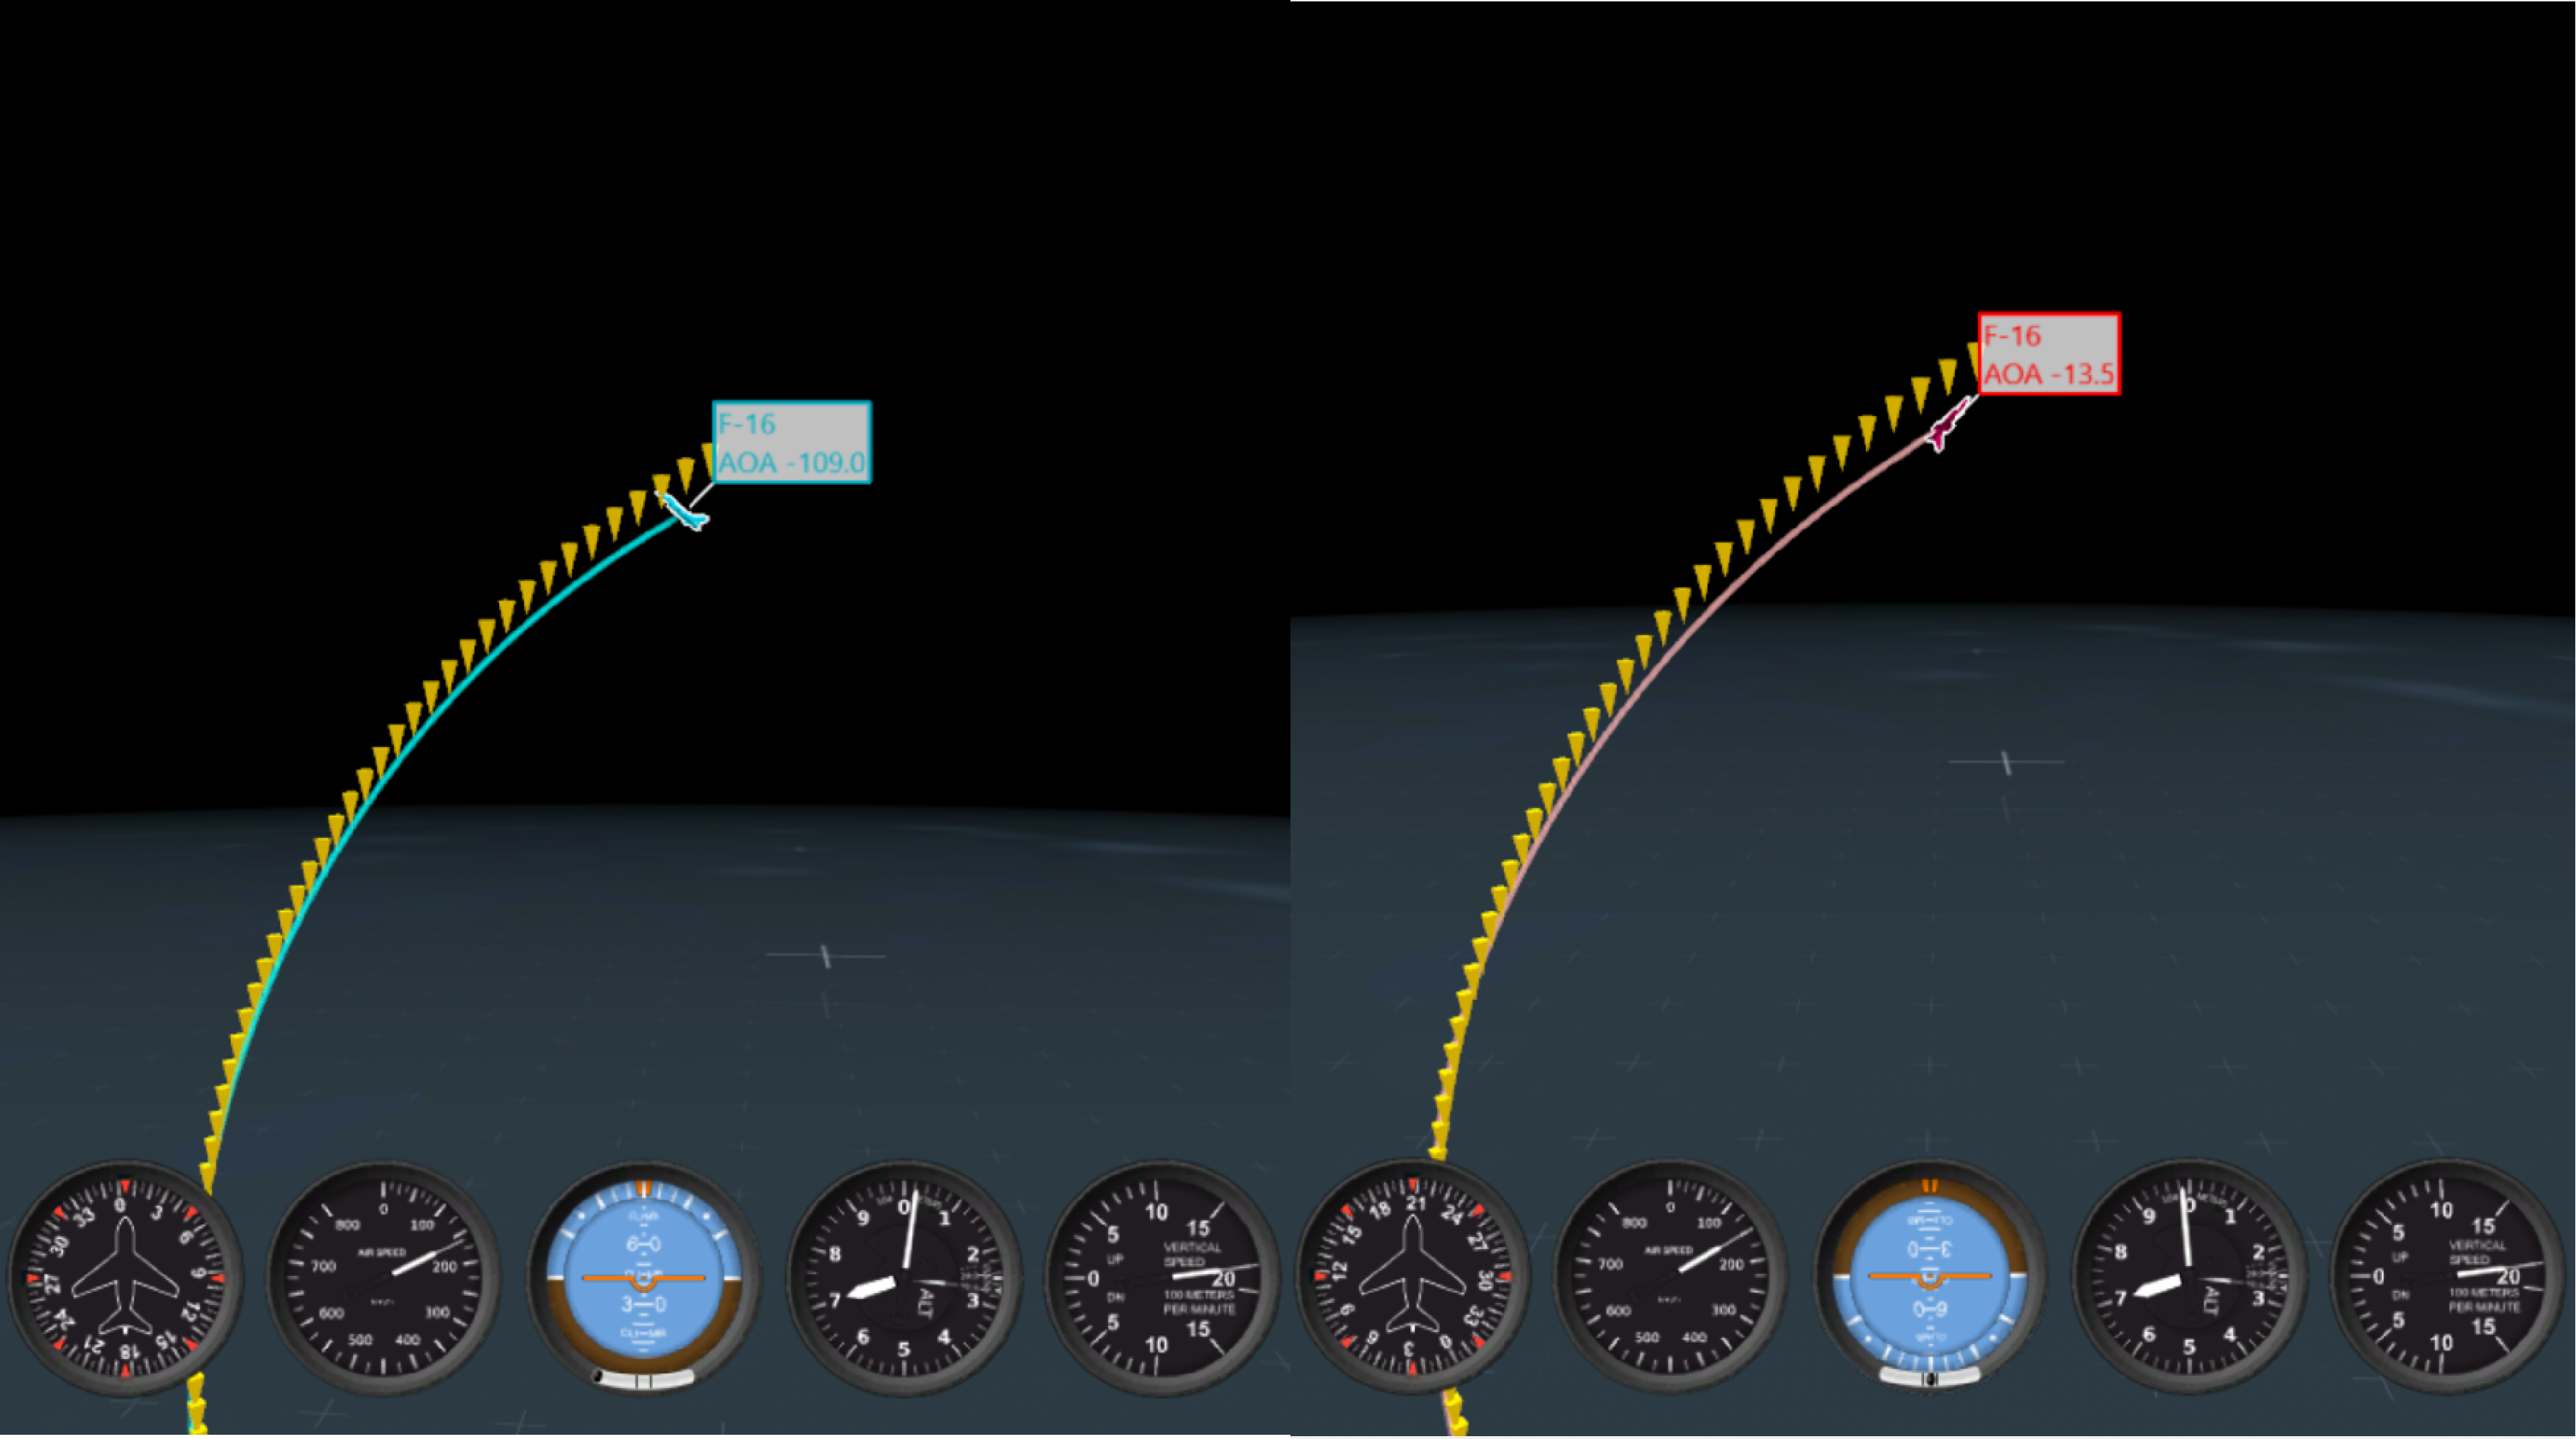
\includegraphics[width=0.98\linewidth]{figure/figure3.png}
    }
  \end{tabular}
  \vspace{-2mm}
  \caption{
  \textbf{Pseudo-tracking diagnosis.}
  Both rollouts remain close to the spatial reference under CTE, but the CTE-only rollout is physically inconsistent because it accumulates unsafe angle-of-attack/energy behavior and poor tangent alignment.
  The energy-aware fine-tuned skill yields a more plausible vertical maneuver with improved velocity--tangent consistency and safety margins.
  }
  \label{fig:pseudo-tracking}
  \vspace{-2mm}
\end{figure}

\begin{table}[t]
  \caption{Energy-aware vertical extension. The fine-tuned vertical skill preserves most original-task survival while correcting catastrophic failures on negative heading changes and reducing stall rates. Each task is evaluated with 10 seeds.}
  \label{tab:vertical-extension}
  \centering
  \small
  \setlength{\tabcolsep}{4pt}
  \begin{tabular}{@{}llccc@{}}
    \toprule
    \textbf{Task}
    & \textbf{Policy}
    & \textbf{Survival}
    & \shortstack{\textbf{Att. Err.}\\\textbf{($^\circ$)}}
    & \shortstack{\textbf{Stall}\\\textbf{Rate}} \\
    \midrule
    \multirow{2}{*}{Level flight}
      & base skill & 1.00 & 7.6 & 0.010 \\
      & fine-tuned vertical skill & 1.00 & 7.3 & 0.002 \\
    \midrule
    \multirow{2}{*}{Heading $+45^\circ$}
      & base skill & 1.00 & 12.8 & 0.000 \\
      & fine-tuned vertical skill & 1.00 & 11.1 & 0.000 \\
    \midrule
    \multirow{2}{*}{Heading $-45^\circ$}
      & base skill & 0.00 & 56.9 & 0.000 \\
      & fine-tuned vertical skill & 1.00 & 11.9 & 0.006 \\
    \midrule
    \multirow{2}{*}{Heading $-20^\circ$}
      & base skill & 0.00 & 62.2 & 0.375 \\
      & fine-tuned vertical skill & 1.00 & 7.8 & 0.000 \\
    \midrule
    \multirow{2}{*}{Circle $R5000$ right}
      & base skill & 1.00 & 11.0 & 0.008 \\
      & fine-tuned vertical skill & 1.00 & 10.8 & 0.000 \\
    \midrule
    \multirow{2}{*}{S-curve $A3000$}
      & base skill & 1.00 & 7.0 & 0.005 \\
      & fine-tuned vertical skill & 1.00 & 7.8 & 0.000 \\
    \midrule
    \multirow{2}{*}{$30^\circ$ pull-up $R8000$}
      & base skill & 1.00 & 17.7 & 0.024 \\
      & fine-tuned vertical skill & 1.00 & 18.7 & 0.006 \\
    \bottomrule
  \end{tabular}
\end{table}


\subsection{Target-Stream Selection}

Table~\ref{tab:stream-and-frontier}(a) reports the closed-loop stream sweep.
Horizontal and mild-3D curves prefer shorter lookahead and lower speed, while the vertical pull-up prefers longer lookahead and higher speed.
This task dependence supports closed-loop stream selection over a single fixed stream parameter.
The selected streams improve CTE-P90 by 39\%, 2\%, 24\%, and 47\% on S-curve, figure-eight, helix, and $90^\circ$ vertical pull-up tasks.

% \begin{table}[t]
%   \caption{Target-stream selection from the closed-loop sweep. Best values are compared with the default stream $(1000~\mathrm{m},250~\mathrm{m/s})$. CTE-P90 is in meters.}
%   \label{tab:stream-results-old}
%   \centering
%   \begin{tabular}{lcccc}
%     \toprule
%     \textbf{Maneuver} & \textbf{Best $(L,\vt^\star)$} & \textbf{Best CTE-P90} & \textbf{Default CTE-P90} & \textbf{Improvement} \\
%     \midrule
%     S-curve & $(600,220)$ & 918 & 1503 & 39\% \\
%     Figure-eight & $(600,220)$ & 1017 & 1039 & 2\% \\
%     Helix / mild-3D & $(600,220)$ & 524 & 691 & 24\% \\
%     $90^\circ$ vertical pull-up & $(1500,280)$ & 51 & 96 & 47\% \\
%     \bottomrule
%   \end{tabular}
% \end{table}


\begin{figure}[t]
  \centering
  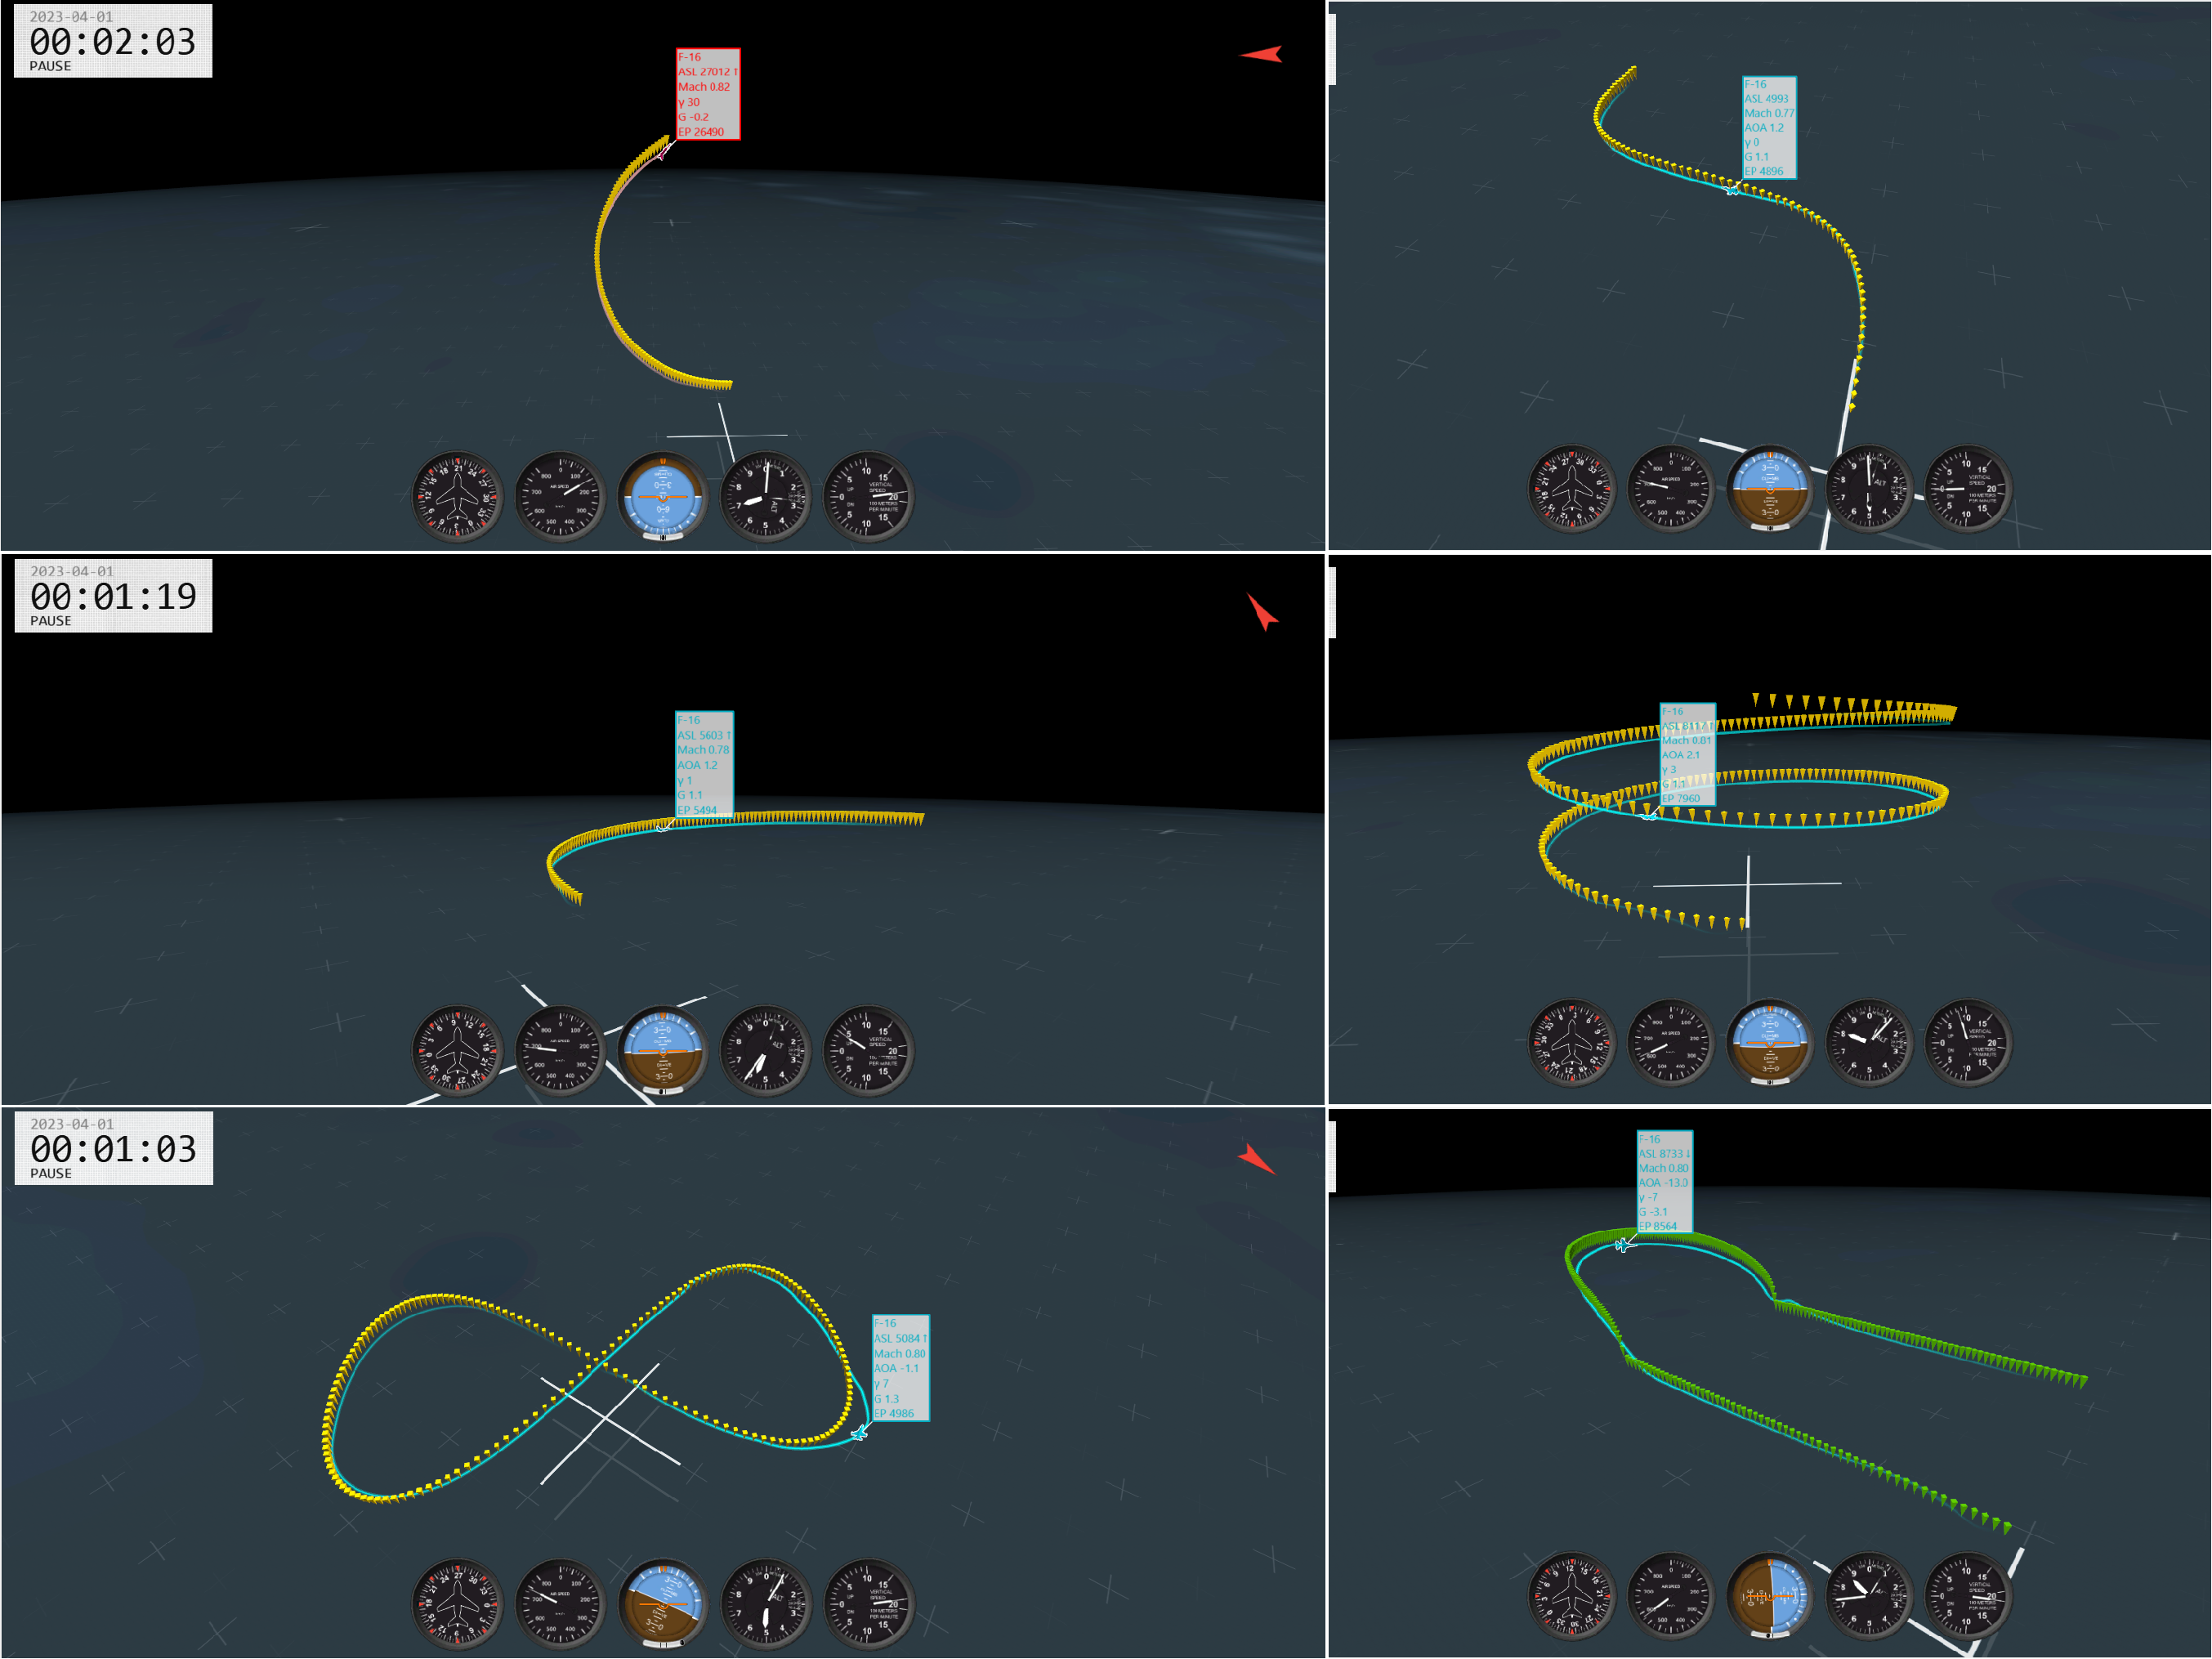
\includegraphics[width=0.84\textwidth,trim=0 8 0 8,clip]{figure/figure2.png}
  \vspace{-2mm}
  \caption{\textbf{Representative maneuver suite.}
  The evaluation covers horizontal, mild-3D, vertical pull-up, and completed loop-like maneuvers.}
  \label{fig:maneuvers}
  \vspace{-3mm}
\end{figure}

\subsection{Demonstrated Maneuvers and Large-Attitude Evaluation}

Figure~\ref{fig:maneuvers} shows executable maneuvers generated by the proposed skill and stream interface, not benchmark-provided demonstrations.
Table~\ref{tab:stream-and-frontier} further reports the large-attitude evaluation.
After energy-aware fine-tuning, the frozen PPO executor can complete vertical-arc maneuvers, and selected target streams further compose the executor into a completed loop-like maneuver.
The remaining errors are therefore better interpreted as execution-quality and energy-margin limitations rather than basic maneuver-completion failures.

% \begin{table}[t]
%   \caption{Loop-quality frontier under geometry-aware evaluation. All metric values are P90 errors. B-grade arcs complete the reference geometry with moderate geometric error; the $180^\circ$ half-loop fails.}
%   \label{tab:loop-frontier}
%   \centering
%   \small
%   \setlength{\tabcolsep}{4pt}
%   \begin{tabular}{@{}lccccc@{}}
%     \toprule
%     \textbf{Arc angle}
%     & \textbf{CTE (m)}
%     & \shortstack{\textbf{Vel.-tan.}\\\textbf{($^\circ$)}}
%     & \shortstack{\textbf{Nose-tan.}\\\textbf{($^\circ$)}}
%     & \shortstack{\textbf{Wing-plane}\\\textbf{($^\circ$)}}
%     & \textbf{Grade} \\
%     \midrule
%     $60^\circ$  & 180.0   & 12.8  & 18.1  & 103.6 & B \\
%     $90^\circ$  & 152.5   & 10.1  & 13.1  & 66.2  & B \\
%     $105^\circ$ & 138.3   & 9.5   & 12.3  & 80.0  & B \\
%     $120^\circ$ & 121.3   & 8.8   & 10.2  & 69.5  & B \\
%     $135^\circ$ & 120.1   & 6.9   & 7.5   & 60.4  & B \\
%     $150^\circ$ & 181.2   & 6.6   & 8.8   & 49.2  & B \\
%     $180^\circ$ & 19515.6 & 140.6 & 131.7 & 162.8 & Fail \\
%     \bottomrule
%   \end{tabular}
% \end{table}
\begin{table}[!t]
\centering
\footnotesize
\setlength{\tabcolsep}{2.6pt}
\renewcommand{\arraystretch}{0.95}
\caption{\textbf{Target-stream selection and large-attitude maneuver evaluation.}
Left: closed-loop target-stream sweep. Right: geometry-aware evaluation of vertical and loop-like maneuvers.}
\label{tab:stream-and-frontier}

\makebox[\linewidth][c]{%
\begin{minipage}[t]{0.50\linewidth}
\centering
\textbf{(a) Target-stream sweep}
\vspace{0.5mm}

\begin{tabular}{@{}lccc@{}}
\toprule
\textbf{Task} & \textbf{Best} & \textbf{CTE} & \textbf{Imp.} \\
\midrule
S-curve & $(600,220)$ & $918/1503$ & 39\% \\
Fig.-8 & $(600,220)$ & $1017/1039$ & 2\% \\
Helix & $(600,220)$ & $524/691$ & 24\% \\
$90^\circ$ PU & $(1500,280)$ & $51/96$ & 47\% \\
\bottomrule
\end{tabular}

\vspace{0.5mm}
{\scriptsize CTE is best/default; default stream is $(1000,250)$.}
\end{minipage}%
\hspace{0.01\linewidth}%
\begin{minipage}[t]{0.47\linewidth}
\centering
\textbf{(b) Large-attitude evaluation}
\vspace{0.5mm}

\begin{tabular}{@{}lcccc@{}}
\toprule
\textbf{Arc} & \textbf{CTE} & \textbf{$e_v$} & \textbf{$e_w$} & \textbf{Grade} \\
\midrule
$60^\circ$  & 180.0   & 12.8  & 103.6 & B \\
$90^\circ$  & 152.5   & 10.1  & 66.2  & B \\
$105^\circ$ & 138.3   & 9.5   & 80.0  & B \\
$120^\circ$ & 121.3   & 8.8   & 69.5  & B \\
$135^\circ$ & 120.1   & 6.9   & 60.4  & B \\
$150^\circ$ & 181.2   & 6.6   & 49.2  & B \\
$Full loop$ & 181.0 & 6.7 & 45.1 & B \\
\bottomrule
\end{tabular}
\end{minipage}%
}

\vspace{-1mm}
\end{table}

%===============================================================================

\section{Discussion and Limitations}

The learned skill is not a full autonomy stack or a real-flight deployment claim; it is a direct-actuator executor with an explicit attitude--speed interface.
Closed-loop stream selection optimizes low-dimensional target-stream parameters rather than actuator sequences, and the deterministic lattice used here is only grid-optimal within the enumerated candidate set.
Richer stream parameterizations could replace the lattice with sampling-based optimizers such as CEM or MPPI~\citep{rubinstein1999cross,williams2017mppi}, while preserving the same executable-stream interface.

The current system should still be interpreted as a simulation-stage aerobatic maneuvering result rather than a real-flight deployment claim.
Energy-aware fine-tuning and selected target streams enable completed loop-like maneuver execution in simulation, but the resulting maneuvers can still exhibit non-negligible wing-plane errors, energy-margin sensitivity, and task-dependent quality variation.
Future work should address wind and state-estimation errors, actuator mismatch, domain randomization, external safety monitoring, and real-flight validation.
Simulation-to-real techniques such as visual and dynamics randomization~\citep{tobin2017domain,peng2018sim}, iterative sim-to-real adaptation~\citep{chebotar2019closing}, and robust policy transfer practices~\citep{hwangbo2019learning} provide useful directions, but real fixed-wing deployment would require additional validation beyond the scope of this paper.

\section{Conclusion}

We presented energy-aware target streams for learned fixed-wing maneuvering.
The framework combines a quaternion-conditioned direct-actuator skill, geometry-aware pseudo-tracking diagnosis, energy-aware capability expansion, and closed-loop executable target-stream selection.
Experiments show that quaternion targets improve complex curve maneuvers, energy-aware fine-tuning improves safety and reliability on vertical-extension tasks, and task-dependent target streams improve CTE-P90 on horizontal, mild-3D, and vertical pull-up maneuvers.
The updated vertical evaluations further show that the fine-tuned PPO executor and selected target streams can complete loop-like large-attitude maneuvers in simulation.
Geometry-aware metrics remain important because they reveal residual quality limitations in velocity alignment, wing-plane consistency, safety margins, and energy management even when the maneuver is completed.

%===============================================================================

\bibliography{example}

\end{document}
